\newpage
\subsection{Поступление материалов}
\label{bp:MatInput}
%


\subsubsection{Поступление бумаги и картона}

Рулоны бумаги и картона принимаются кладовщиками на склад ролевой продукции. 

Сырье транспортируется машинами. При срочной необходимости могут с предприятия <<Эколайнер>>  привезти автопогрузчиком необходимый рулон. 

Сырье с <<Эколайнер>> поступает по актам передачи (рис. \ref{pic:f13}). Их подписывают кладовщики. Сырье других поставщиков приходит с обычным пакетом документов. 

При поступлении сырья на склад кладовщик сверяет данные, указанные на маркировочных этикетках рулонов с сырьем, с данными, указанными в документах (рис. \ref{pic:f9}), вносит данные в таблицу MS EXCEL (рис. \ref{pic:f1}), где ведется основной учет. 

Основные документы сразу поступают в бухгалтерию.





% \subsubsection{Поступление рулонов бумаги и картона}

% Не производится.




\subsubsection{Поступление прочих материалов}

На момент обследования все вспомогательные материалы числятся на складе другого завода.



\begin{figure}
\begin{center}
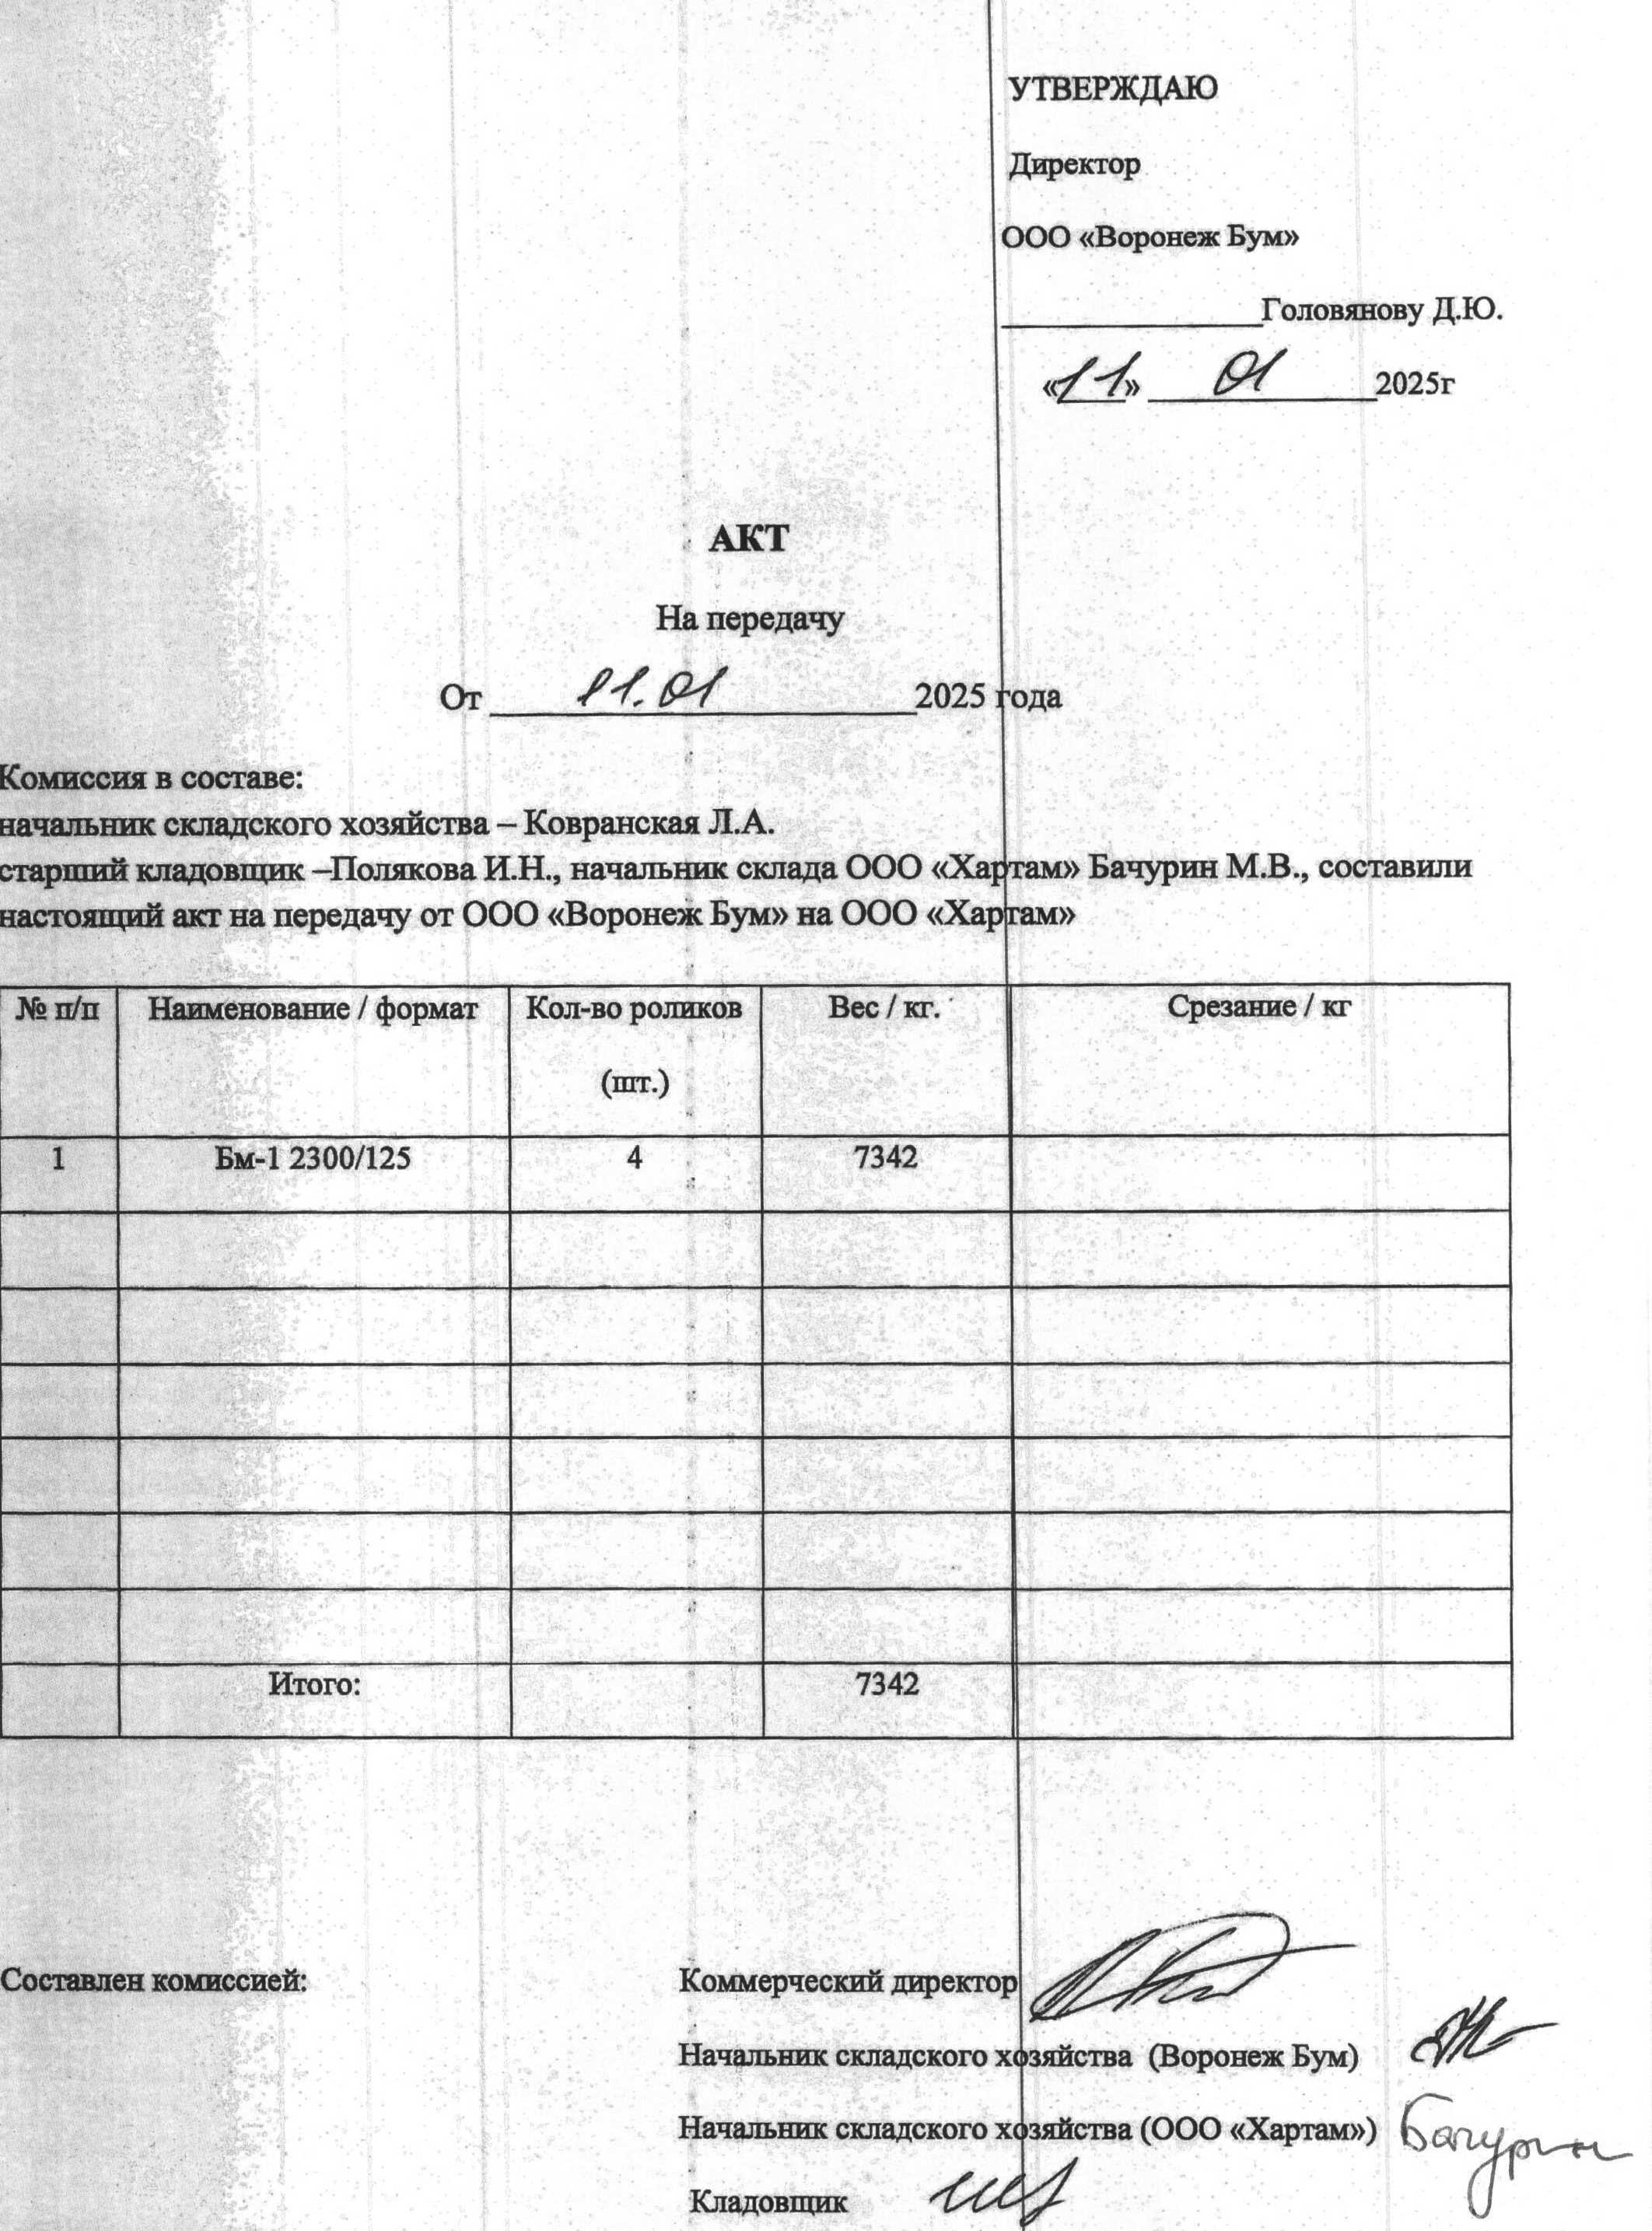
\includegraphics[height=0.94\textheight, width=\textwidth, keepaspectratio]{Pics/f13.jpg}
\end{center}
\caption{Акт на передачу}
\label{pic:f13}
\end{figure}

\begin{figure}
\begin{center}
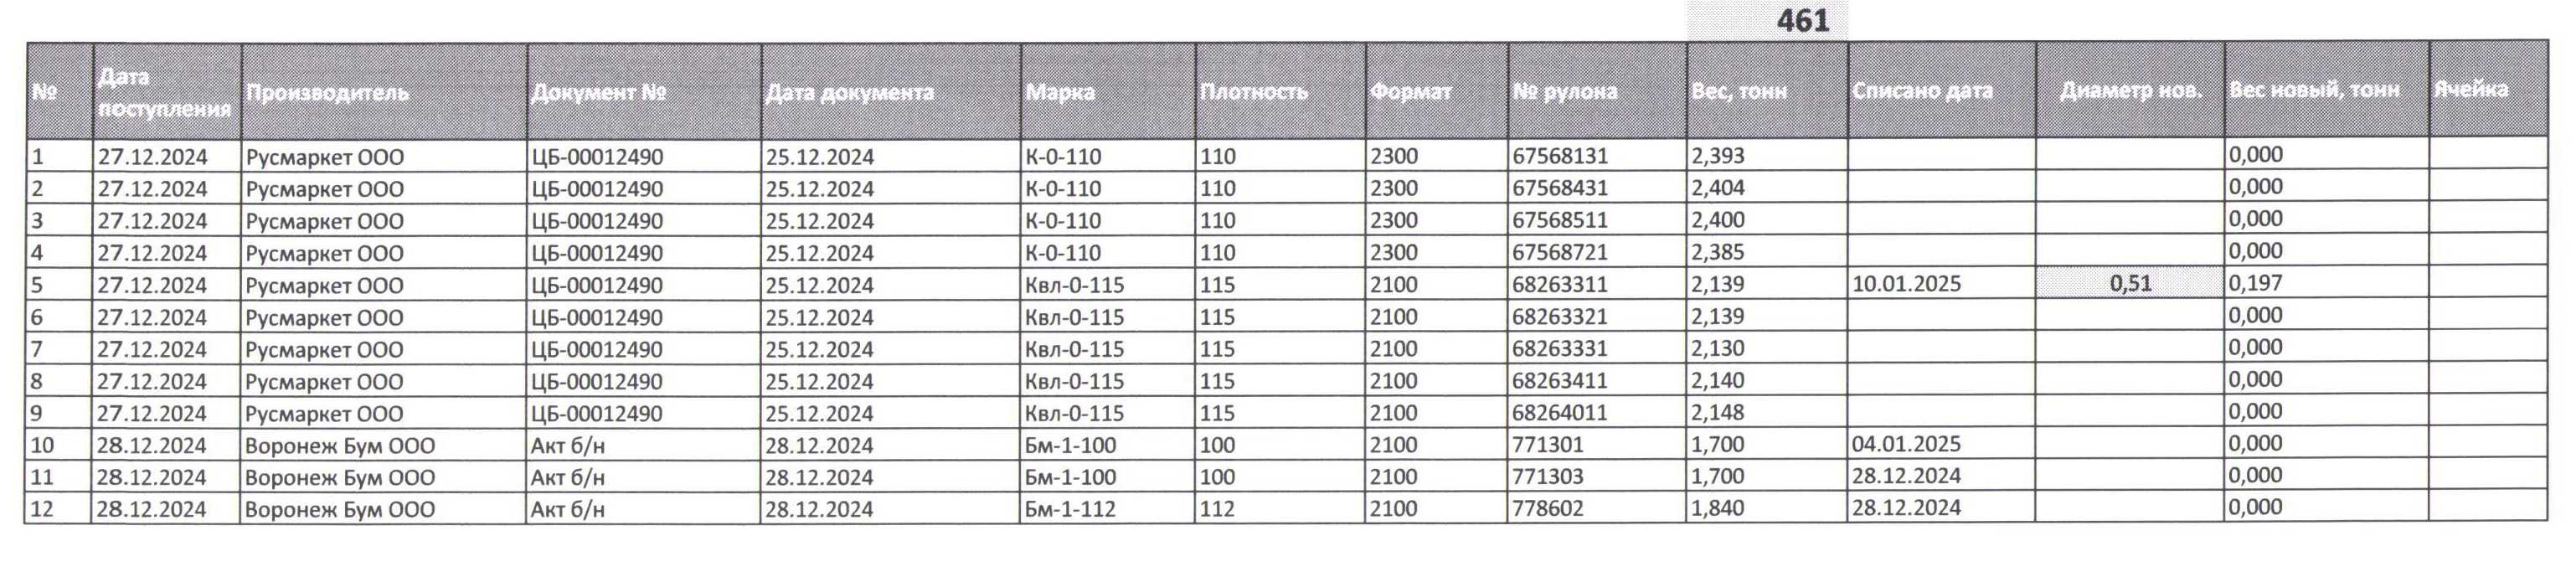
\includegraphics[height=0.94\textheight, width=\textwidth, angle=90, keepaspectratio]{Pics/f1.jpg}
\end{center}
\caption{По рулонный учет сырья}
\label{pic:f1}
\end{figure}

\begin{figure}
\begin{center}
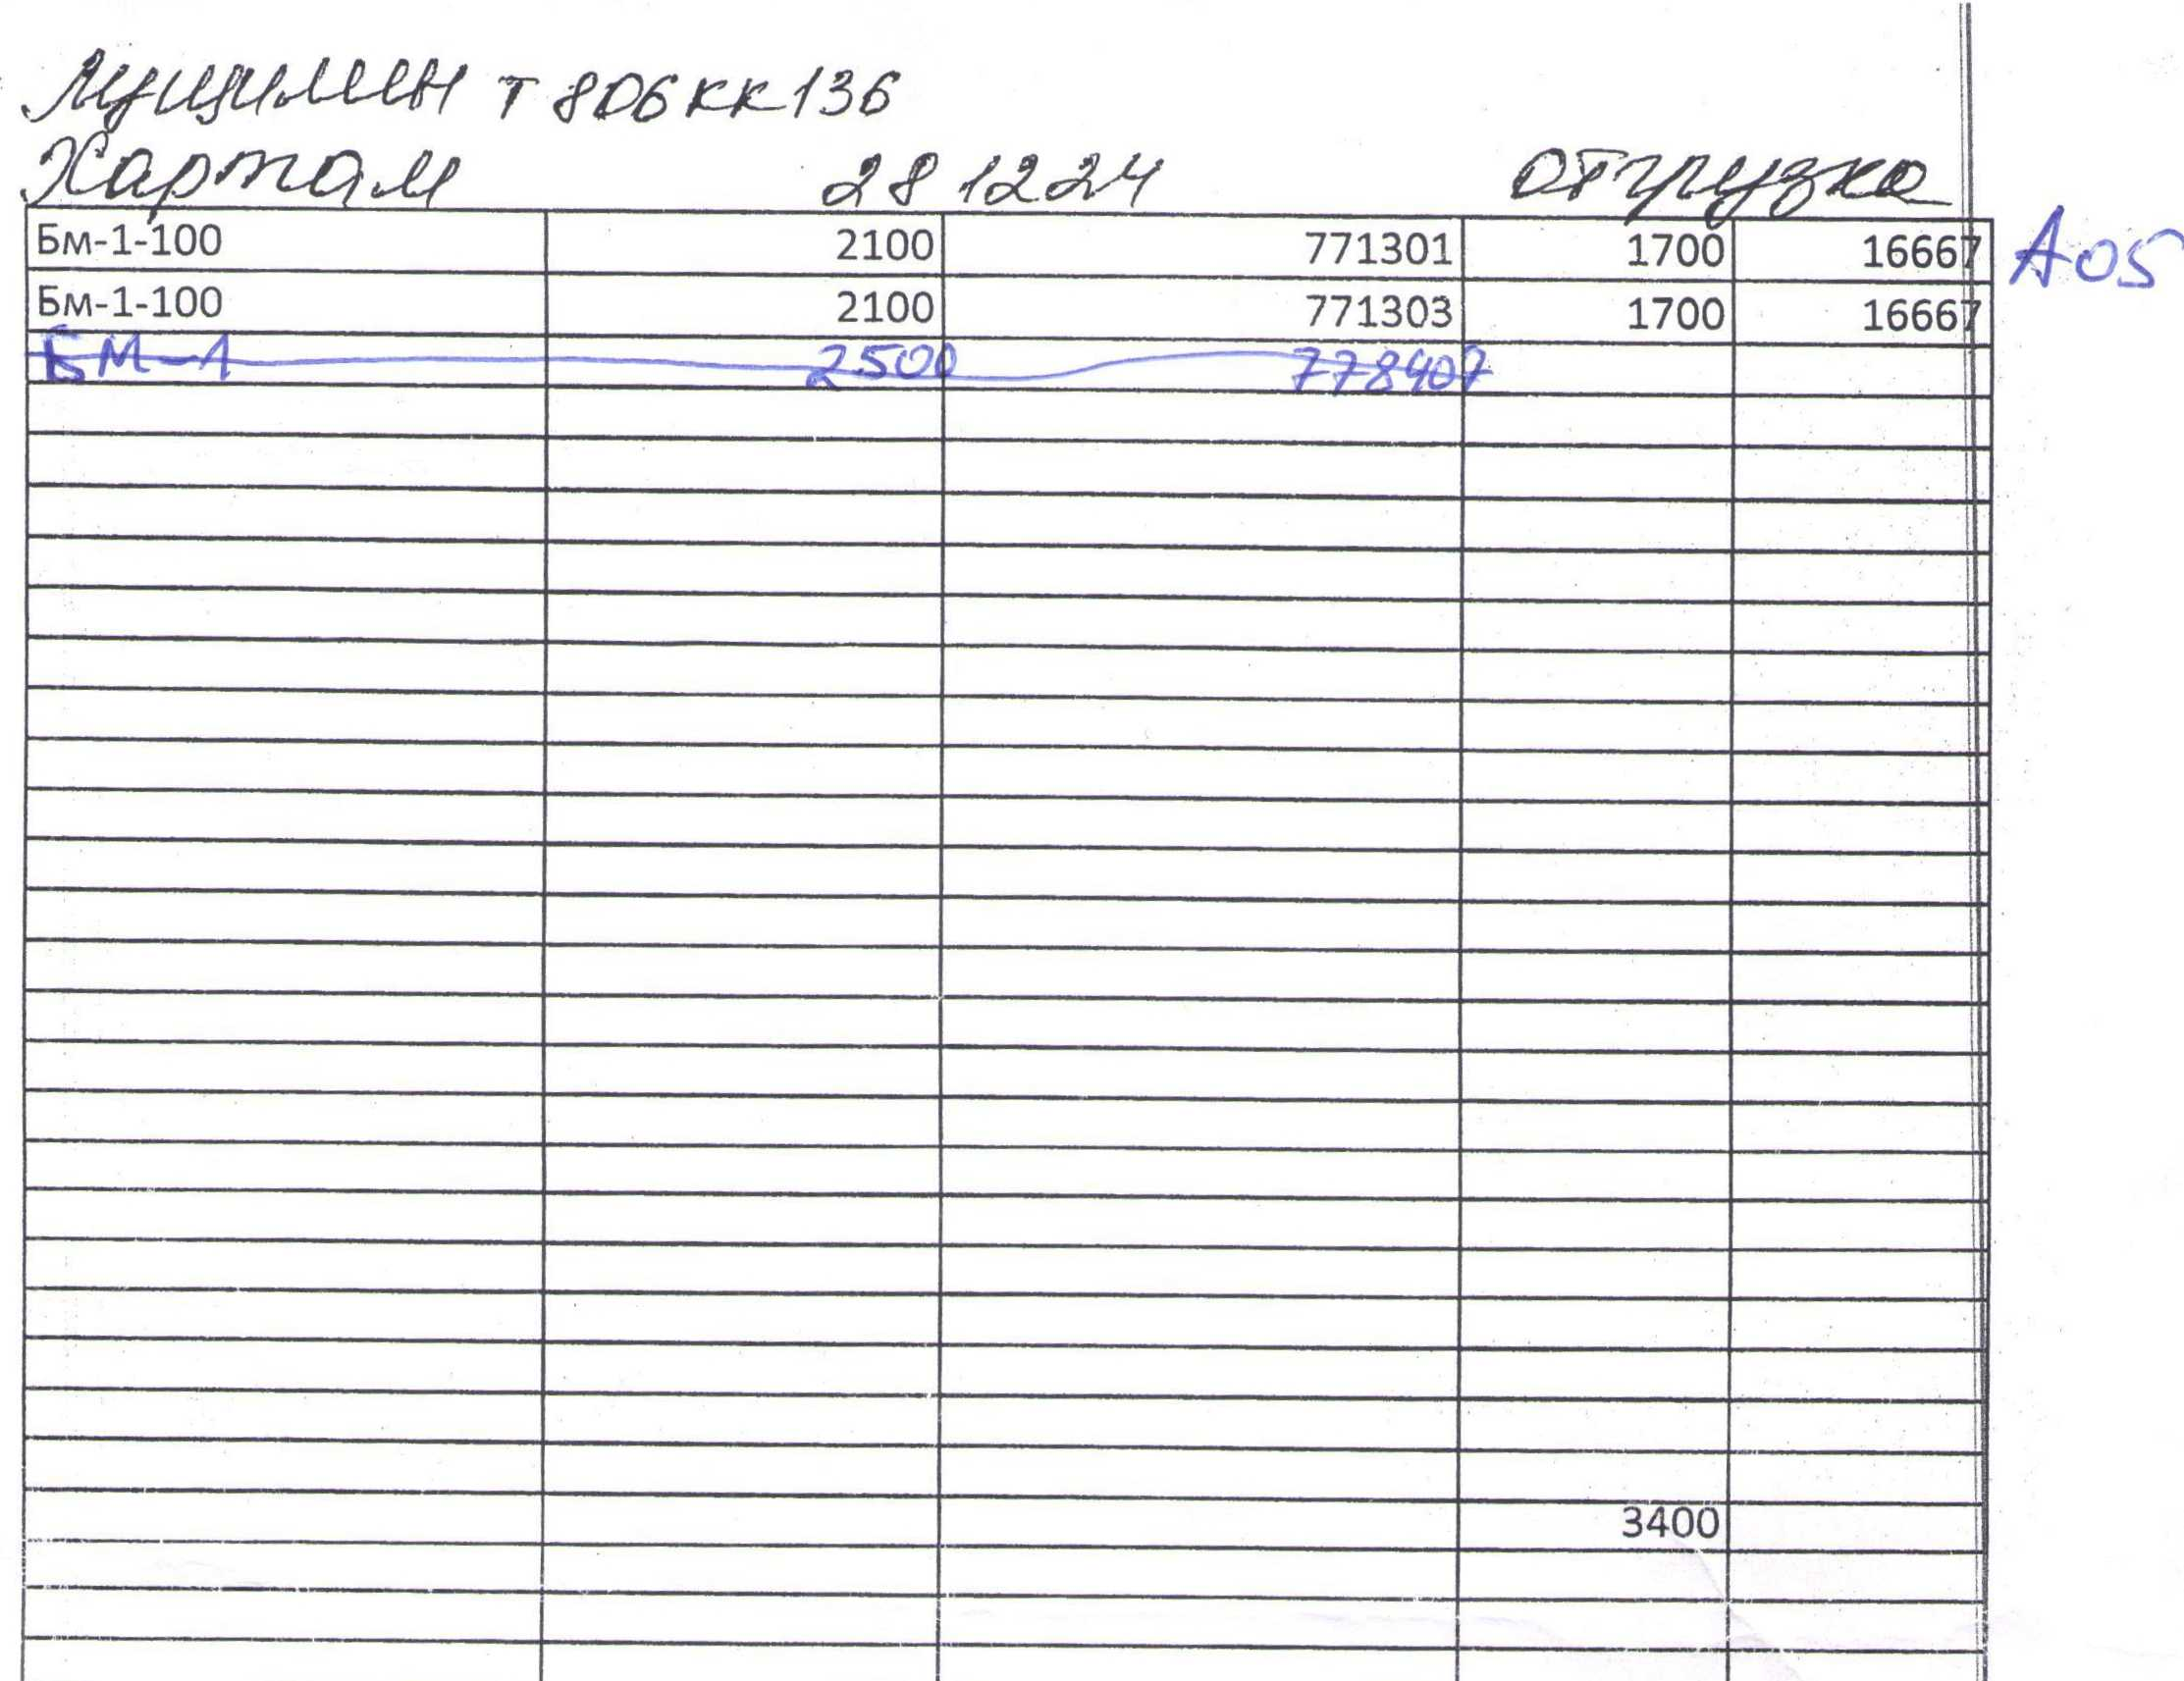
\includegraphics[height=0.94\textheight, width=\textwidth, angle=90, keepaspectratio]{Pics/f9.jpg}
\end{center}
\caption{Отвес сырья}
\label{pic:f9}
\end{figure}


\clearpage
\ifx \notincludehead\undefined
\normalsize
\end{document}
\fi